

\begin{figure*} [t]
\center
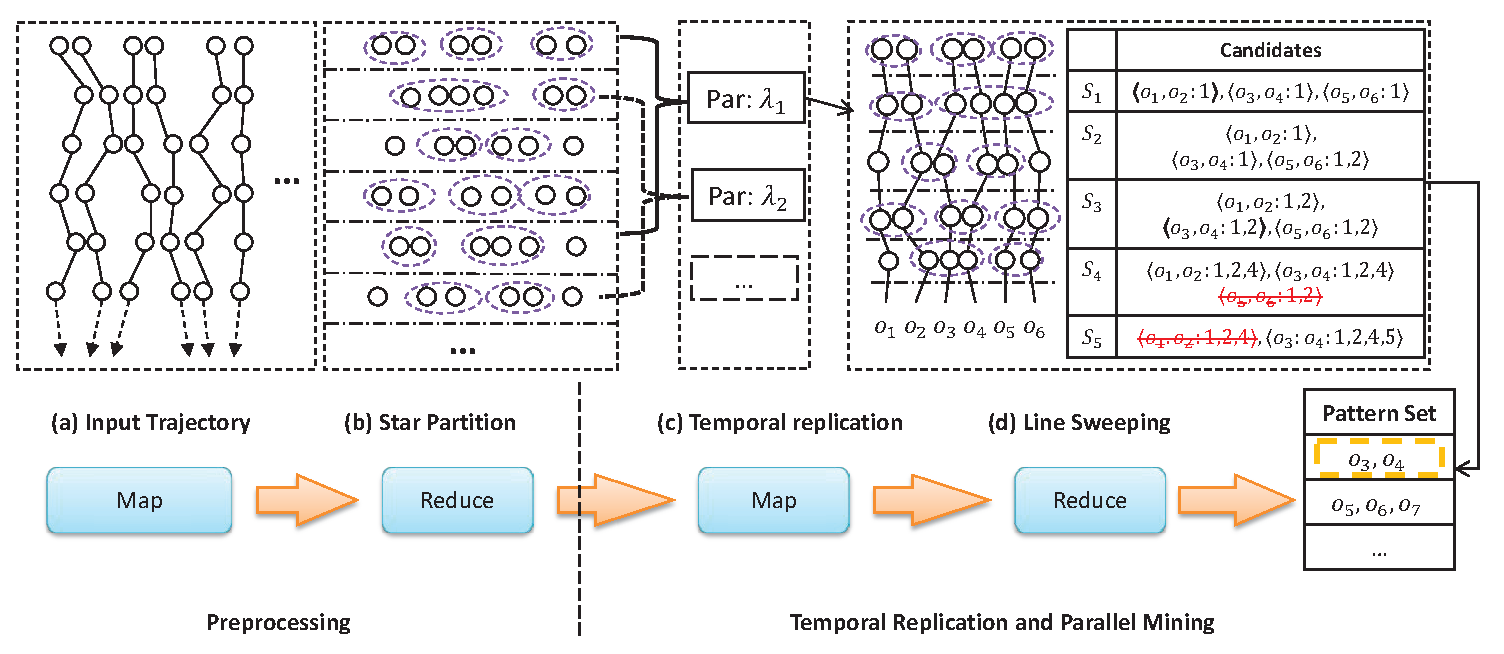
\includegraphics[width=\textwidth]{trm.eps}
\caption{Work flow of Temporal Replication and Parallel Mining. (a)(b) correspond to the first map-reduce cycle which clusters objects in each snapshot;  (c)(d) correspond to the second map-reduce cycle uses TRPM to detect GCMP in parallel.}
\label{fig:trm}
\end{figure*}

\section{Baseline: Temporal Replication and Parallel Mining}
\label{sec:trm}
In this section, we propose a baseline solution that resorts to MapReduce (MR) as a general, parallel and scalable paradigm for GCMP pattern mining. The framework, named \textit{temporal replication and parallel mining} (TRPM), is illustrated in   Figure~\ref{fig:trm}. There are two cycles of map-reduce jobs connected in a pipeline manner. The first cycle deals with spatial clustering in each snapshot, which can be seen as a preprocessing step for the subsequent pattern mining. In particular, the timestamp is treated as the key in the map phase and objects within the same snapshot are clustered (DBSCAN or disk-based clustering) in the reduce phase. Finally, the reducers output clusters of objects in each snapshot, represented by a list of $\langle t,S_t \rangle$ pairs, where $t$ is the timestamp and $S_t$ is a set of clustered objects at snapshot $t$. 

Our focus in this paper is the second map-reduce cycle of parallel mining, which essentially consists of two key questions to solve. The first is how to employ effective data partitioning such that the mining can be conducted independently; and the second is how to efficiently mine the valid patterns within each partition. 


It is obvious that we cannot simply split the trajectory database 
into disjoint partitions because a GCMP pattern requires $L$-consecutiveness 
and the corresponding segments may cross multiple partitions. 
Our strategy is to use data replication to enable parallel mining. 
Each snapshot will replicate its clusters to $\eta-1$ preceding snapshots.
In other words, the partition for the snapshot $S_t$ contains clusters 
in $S_t$, $S_{t+1}\ldots,S_{t+\eta-1}$. 
Determining a proper $\eta$ is critical in ensuring the
correctness and efficiency of TRPM. If $\eta$ is too small, 
certain cross-partition patterns may be missed. 
If $\eta$ is set too large, expensive network communication and 
CPU processing costs would be incurred in the map and reduce phases respectively. Our objective is to find an $\eta$ that is not large but can guarantee correctness.


In our implementation, we set $\eta = (\lceil \frac{K}{L} \rceil - 1)*(G-1)+K+L-1$. Intuitively, $K$ timestamps generates at most $\lceil \frac{K}{L} \rceil - 1$ gaps as the length of each $L$-consecutive segment is at least $L$. Since the gap size is at most $G-1$, $(\lceil \frac{K}{L} \rceil - 1)*(G-1)$ is the upper bound of timestamps allocated to gaps. The remaining part $K+L-1$ is used to capture the upper bound allocated for the $L$-consecutive segments. We formally prove that $\eta$ can guarantee correctness.


\eat{
Before moving on to find the value of $\eta$, 
we first use $\rho_{G,L,K}(T)$ to define the \emph{min-spanned valid subsequence} 
of a sequence $T$. In simple words, $\rho_{G,L,K}(T)$ is the 
subsequence of $T$ with the smallest range and is valid wrt. $K,L,G$. 
%Let $\eta_T$ denote
%the range of $\rho_{G,L,K}(T)$.
To guarantee that no valid patterns are missing, $\eta$ needs
to be greater than the range of $\rho_{G,L,K}(T)$ for any
valid sequence $T$. To see this, consider an arbitrary valid sequence $T$.
Since each partition contains $\eta$ snapshots,
if $\eta \geq \range(\rho_{G,L,K}(T))$ holds, $\rho_{G,L,K}(T)$ must be completely located in one partition. Therefore, the patterns associated with $T$ would not be missing.
Formally, $\eta$ can be computed as:
\begin{equation}
\eta = \max\{\range(\rho_{G,L,K}(T)) | T \text{ is valid wrt. } G,L,K\}
\end{equation}

Directly compute such $\eta$ is challenging. However,
we provide the following theorem which states a bounded estimation on $\eta$: 
}



\begin{theorem}
\label{THM:RP_ETA}
$\eta = (\lceil \frac{K}{L} \rceil - 1)*(G-1)+K+L-1$ guarantees that no valid pattern is missing.
\end{theorem}
\begin{proof}
Given a valid pattern $P$, we can always find at least one valid subsequence that is also valid. Let $T'$ denote the valid subsequence with the minimum length. In the worst case, $T'=P.T$. We define $\range(T)=\max(T) - \min(T) +1$ and prove the theorem by showing that $\range(T') \leq \eta$.
Since $T'$ can be written as a sequence of L-consecutive segments interleaved by gaps: $l_1,g_1,\ldots,l_{n-1},g_{n-1},l_n$ ($n \geq 1$),
where $l_i$ is a segment and $g_i$ is a gap. Then, $\range(T')$
is calculated as $\Sigma_{i=1}^{i=n}|l_i| + \Sigma_{i=1}^{i=n-1} |g_i|$. Since $T'$
is valid, then $\Sigma_{i=1}^{i=n}|l_i| \geq K$. As $T'$ is minimum, if we remove the 
last $l_n$, the resulting sequence should not be valid. Let $K' = \Sigma_{i=1}^{i=n-1}|l_i|$, which
is the size of the first $(n-1)$ segments of $T'$. Then, $K' \leq K-1$.
Note that every $|l_i| \geq L$, thus $n \leq \lceil \frac{K'}{L} \rceil \leq \lceil \frac{K}{L} \rceil $. By
using the fact that every $|g_i| \leq G-1$, we achieve $\Sigma_{i=1}^{i=n-1} |g_i| \leq (n-1)(G-1)
\leq (\lceil \frac{K}{L} \rceil -1)(G-1)$. Next, we consider the difference between $K$ and $K'$, denoted by
$\Delta = K- K'$. To ensure $T'$'s validity, $l_n$ must equal to $\min(L, \Delta)$.
Then, $\Sigma_{i=1}^{i=n}|l_i| = K' + l_n = K - \Delta + \min(L, \Delta) \leq K - 1 + L$. We finish showing $\range(T') \leq \eta$.  Therefore, for any valid sequence $T$, it exists at least one valid subsequence with range no greater than $\eta$ and hence this pattern can be detected in a partition with $\eta$ snapshots.
\end{proof}

\eat{
Note that Theorem~\ref{THM:RP_ETA} does not state the optimal value of $\eta$
for a given $G,L,K$. However, for any $G,L,K$, $\eta$ does not differ from
the optimal value by at most $L-1$. To see this, for any $G,L,K$, we can
generate a sequence $T$ by repeating the following pattern, a $L$-segment followed by $G$-gap. 
The repetition stops when $|T|\geq K$. Apparently $T$ is valid wrt. $G,L,K$.
It is easy to see that $T$ is minimal valid subsequence of itself, then $\eta^*  \geq \range(T) \geq (\lceil \frac{K}{L}\rceil -1)(G-1) + K$.
Therefore $\eta-\eta^* \leq L-1$.
}

\begin{algorithm}[h]
\caption{Line Sweep Mining}
\label{algo:line-sweep}
\begin{algorithmic}[1]
\Require $\lambda_t = \{S_t, ..., S_{t+\eta-1}\}$
\State{$C \gets \{\}$} \Comment{Candidate set} \label{code:ls-can-set}
\ForAll{clusters $s$ in snapshot $S_t$} 
\label{code:ls-init-start}
\If{$|s| \geq M$}
\State $C\leftarrow C\cup \{\langle s, t \rangle \}$
\EndIf
\EndFor
\label{code:ls-init-end}
\ForAll{$S_j \in \{S_{t+1},\ldots,S_{t+\eta-1}\}$} \label{code:ls-sweep-starts}
	\State $N \gets \{\}$
	\ForAll {$(c,s) \in C \times S_j$} \label{code:ls-join-start}
		\State {$c' \gets \langle c.O \cap s.O, c.T \cup \{j\} \rangle$} \label{code:ls-join}
		\If {$c'.T$ is valid} 
			\State output $c'$
		\ElsIf{$|c'.O| \geq M$}
			\State $N\leftarrow N\cup \{c'\}$ \label{code:ls-m-prun}	
		\EndIf
	\EndFor \label{code:ls-join-ends}
	\ForAll {$c \in C$}
		\If{$j-\max(c.T)\geq G$}\label{code:ls-g-prune-starts}
			\State $C\leftarrow C-\{c\}$ 
			\State output $c$, if $c$ is a valid pattern
		\EndIf  \label{code:ls-g-prune-ends}
		\If{$c$'s first segment is less than $L$}\label{code:ls-l-prune-starts}
			\State $C\leftarrow C-\{c\}$ 
		\EndIf\label{code:ls-l-prune-ends}
	\EndFor
	\State $C\leftarrow C\cup N$
\EndFor\label{code:ls-sweep-ends}
\State output valid patterns in  $C$  \label{code:ls-valid-check}
\end{algorithmic}
\end{algorithm}



Based on the above theorem, during TRPM, every consecutive $\eta$ snapshots
form a partition. In other words, each snapshot $S_t$ corresponds to a partition $\lambda_t=\{S_t,...,S_{t+\eta-1}\}$. Our next task is to design an efficient pattern mining strategy within each partition. We propose a line sweep algorithm to sequentially scan the $\eta$ replicated snapshots in a partition and employ effective candidate pattern enumeration.  

Details of the algorithm are presented in Algorithm~\ref{algo:line-sweep}. We keep a candidate set $C$ (Line~\ref{code:ls-can-set}) during the sweeping process. It is initialized as the candidate clusters with size no smaller than $M$ in the first snapshot. Then, we sequentially scan each snapshot (Lines~\ref{code:ls-sweep-starts}-\ref{code:ls-sweep-ends}) and generate new candidates by extending the original ones in $C$.
In particular, we join candidates in $C$ with all the clusters in $S_j$ to form new candidates (Lines~\ref{code:ls-join-start}-\ref{code:ls-join-ends}). 
%The join of candidate $c$ and cluster $s$ creates a
%new candidate $c'$ (Line~\ref{code:ls-join}).  
After sweeping all the snapshots, all the valid patterns are stored in $C$(Line~\ref{code:ls-valid-check}). 
It is worth noting that $C$ continues to grow during the whole sweeping process. We can use three pruning rules to 
early remove false candidates from $C$. Since there is a partition $\lambda_t$ for each $S_t$, 
in line sweep, only patterns that starts from timestamp $t$ (i.e., $S_t$) need to be discovered. Therefore, those patterns that does not appear in the $S_t$ are false candidates. Particularly, our
three pruning rules are as follows:
First, when sweeping snapshot $S_j$, new candidates with objects set smaller than $M$ are pruned (Line~\ref{code:ls-m-prun}). Second, after joined with all clusters in $S_j$, 
candidates in $C$ with the maximum timestamp no greater than $j-G$ are pruned (Lines~\ref{code:ls-g-prune-starts}-\ref{code:ls-g-prune-ends}). Third, candidates in $C$ with the size of first segment smaller than $L$
are pruned (Lines~\ref{code:ls-l-prune-starts}-\ref{code:ls-l-prune-ends}). With the three pruning rules, the size of $C$ could be significantly reduced.  

%ADD EXPLANATIONS TO THE SECOND AND THIRD PRUNING RULES.

%After join, there are two prunings. First, 
%all new candidates with objects set less than $M$ are pruned (Line~\ref{code:ls-m-prun}). Second,
%existing candidates with max time sequences no greater 
%than $j-G$ are pruned (Line~\ref{code:ls-m-prun}). 
% 
%
%During the sweeping, candidates in $\mathbf{C}$ join with $S_j$.
%
% Initially, all the clusters 
%
%During scanning, a set of pattern candidates is maintained.
%When all snapshots are scanned, the remaining candidates are the true patterns.
%The detail of LSM is presented in Algorithm~\ref{algo:line-sweep}.
%A candidate set $C$ is maintained throughout the algorithm(line~\ref{code:ls-can-set}). $C$
%is initialized by inserting clusters at $S_t$ (lines~\ref{code:ls-init-start}-\ref{code:ls-init-end}).
%During scanning snapshot $S_j$, candidates in $C$ are joined with clusters at $S_j$. In
%the join, a candidate grows its temporal sequence while potentially reduces its object set. After the join,
%false patterns are deleted (line~\ref{code:ls-remove}). 
%Note that the size of $C$ is always decreasing, therefore the complexity of LSM $\lambda_t$ is $O(\eta|S_t||\overline{S}|)$,where $|\overline{S}|$ is the average snapshot size in $\lambda_t$.

The complete picture of temporal replication and parallel mining is summarized in Algorithm~\ref{algo:trm_overview}. We illustrate the workflow of TRPM method using Figure~\ref{fig:trm} (c)(d) with pattern
parameters $M=2, K=3, L = 2, G=2$. By Theorem~\ref{THM:RP_ETA}, $\eta$ is calculated
as $(\lceil \frac{K}{L} \rceil-1) *(G-1)+2K - 2 = 5$. Therefore, 
in Figure~\ref{fig:trm} (c), every $5$ consecutive snapshots are combined 
into a partition in the map phase. In Figure~\ref{fig:trm} (d), a line sweep
method is illustrated for partition $\lambda_1$. Let $C_i$ be the candidate set
during sweeping snapshot $S_i$.
Initially, $C_1$ contains patterns with object sets in snapshot $S_1$.
As we sweep the snapshots, the patterns in $C_i$ grow. At snapshot $S_4$, the candidate
$\{o_5,o_6\}$ is removed. This is because the gap between its latest timestamp (i.e., $2$)
and the next scanning timestamp (i.e., $5$) is $3$, which violates the $G$-connected constraint.
Next, at snapshot $S_5$, the candidate $\{o_1,o_2\}$ is removed. This is
because its local consecutive segment $\{4\}$ has only $1$ element,
which violates the $L$-consecutive constraint.
Finally, $\{o_3,o_4\}$ is the valid pattern and is returned. Note that in this example, $\eta=5$ is the minimum setting that can guarantee correctness. If $\eta$ is set to $4$, the pattern $\{o_3,o_4\}$ would be missed. 

\begin{algorithm}[h]
\caption{Temporal Replication and Parallel Mining}
\label{algo:trm_overview}
\begin{algorithmic}[1]
\Require list of $\langle t, S_t \rangle$ pairs
\State $\eta \gets (\lceil \frac{K}{L} \rceil -1)*(G-1)+K+L-1$
\State {---Map Phase---}
\label{code:trm-map-start}
\ForAll{snapshots $S_t$}
	\ForAll{$i \in 1...{\eta-1}$}
		\State emit key-value pair $\langle \max(t-i,0), S_t \rangle$ 
	\EndFor  
\EndFor
\label{code:trm-map-end}
\State {---Partition and Shuffle Phase---}
\label{code:trm-par-start}
\ForAll{key-value pairs $\langle t, S \rangle$ pair} 
\State group-by $t$ and emit a key-value pair $\langle t, \lambda_t\rangle$, where $\lambda_t = \{S_t, S_{t+1}, .. S_{t+\eta-1}\} $
\EndFor
\label{code:trm-par-end}
\State {---Reduce Phase---}
\label{code:trm-red-start}
\ForAll{key-value pairs $\langle t,\lambda_t \rangle$}
\State call line sweep algorithm for partition $\lambda_t$
\label{code:trm-red-end}
\EndFor
\end{algorithmic}
\end{algorithm}
